\begin{frame}{Conclusão}
	\begin{columns}
		\column{0.4\textwidth}
		\begin{minipage}[c][0.4\textheight][c]{\linewidth}
			\centering
			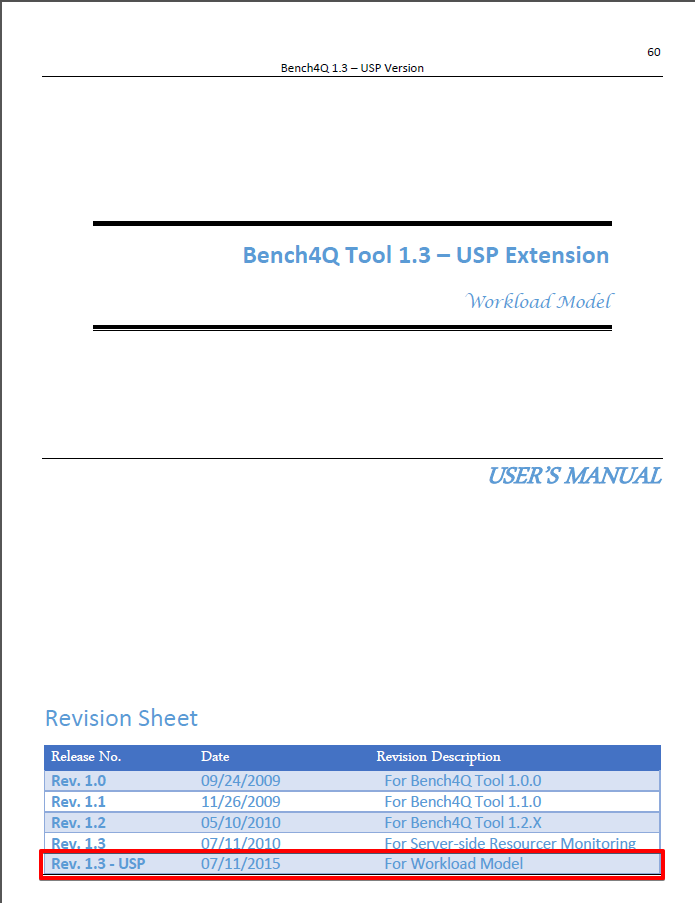
\includegraphics[width=1\linewidth]{images/capa-documentacao.png}
			\label{fig:documentacao}	
		\end{minipage}
		\column{0.6\textwidth}
		\begin{minipage}[c][0.4\textheight][c]{\linewidth}
			\begin{itemize}
				\item A extensão feita no \textit{benchmark}, o Bench4Q, for capaz de modelar a carga de trabalho atendendo o requisito \textit{Demand} do MEDC.
				
				\item A elaboração de uma documentação padronizada da mesma forma que a original do Bench4Q;
				
				\item Impacto da carga modulada: mediante a modulação da carga através da extensão, é possível excitar o sistema a apresentar a sua dinâmica, contribuindo para trabalhos que tem por necessidade a modelagem do sistema e do seu comportamento dinâmico;
			\end{itemize} 
		\end{minipage}		
	\end{columns}	
\end{frame}

%\begin{frame}{Contribuição}
%	\begin{itemize}
%		\item Dinâmica entre camadas: ao se tratar de um sistema de multicamadas, foi possível perceber, juntamente com a modulação da carga, a dinâmica intrínseca entre as camadas do sistema. Os efeitos combinados de atrasos intrínsecos, ainda que pequenos, e sua propagação por todo as camadas interligados geraram um comportamento dinâmico significante e apreciável;
%		
%		\item Métrica que mascara: por consequência da dinâmica inerente ao sistema multicamadas, foi possível vislumbrar que nem toda métrica apresenta a realidade quando se lida com um sistema multicamadas. Neste trabalho, foi possível observar esse fato na métrica tempo de resposta.
%	\end{itemize} 
%\end{frame}

%\begin{frame}{Trabalhos futuros}
%	\begin{itemize}
%		\item \textbf{Novas formas de pertubação:} com base nas proposta de \cite{Hellerstein2004} existem outras funções que auxiliam a excitar o sistema a apresentarem a sua dinâmica. 
%		
%		\item \textbf{Avaliação da dinâmica em sistemas multicamadas:} com o presente trabalho, foi possível observar a dinâmica entre as camadas do sistema, entretanto o presente trabalho não cobre com um planejamento de experimentos utilizando métodos estatísticos por meio de avaliações de desempenho
%		
%		\item \textbf{Avaliação de métricas de planejamento de recursos em ambiente multicamadas:} este trabalho também revelou que existem métricas que podem mascarar a realidade, neste contexto é importante uma análise das principais métricas de diferentes técnicas para o planejamento de recursos sob um ambiente de multicamadas
%	\end{itemize} 
%\end{frame}